\section[Intro]{Introduction and Motivation}
\begin{frame}{Introduction}
\begin{columns}
  \begin{column}{.5 \textwidth}
    \begin{itemize}
      \item global avg. temperature rising $\subset$ climate change 
      \item climate change has a lot of complicated consequences (air pressure, winds, oceans \dots)  
    \end{itemize}
    
    
  \end{column}
  \begin{column}{.5 \textwidth}
    \begin{figure}[t]
      \centering
      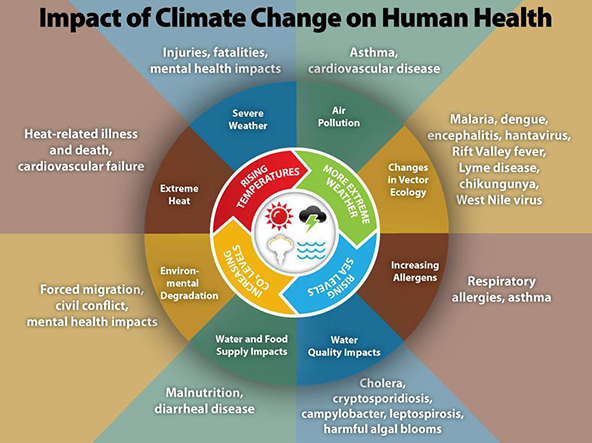
\includegraphics[width=\columnwidth]{imglib/climate_change_health_impacts.jpg}
    \end{figure}
    
  \end{column}
  
\end{columns}
\end{frame}

\begin{frame}{Example: Change of North Atlantic Oscillation}

  \begin{columns}
    \begin{column}{.5 \textwidth}
    See \citeauthor{vietinghoff_visual_2021} \cite{vietinghoff_visual_2021}
    \begin{figure}[t]
      \centering
      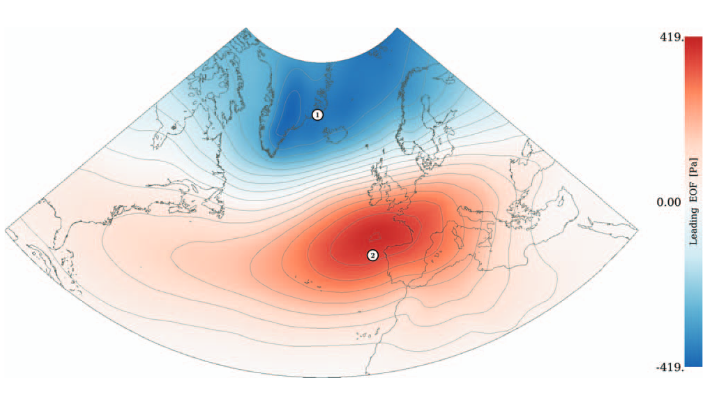
\includegraphics[width=\columnwidth]{imglib/nao_eof_index.png}
    \end{figure}
      
    \end{column}
    \begin{column}{.5 \textwidth}
    \begin{figure}[t]
      \centering
      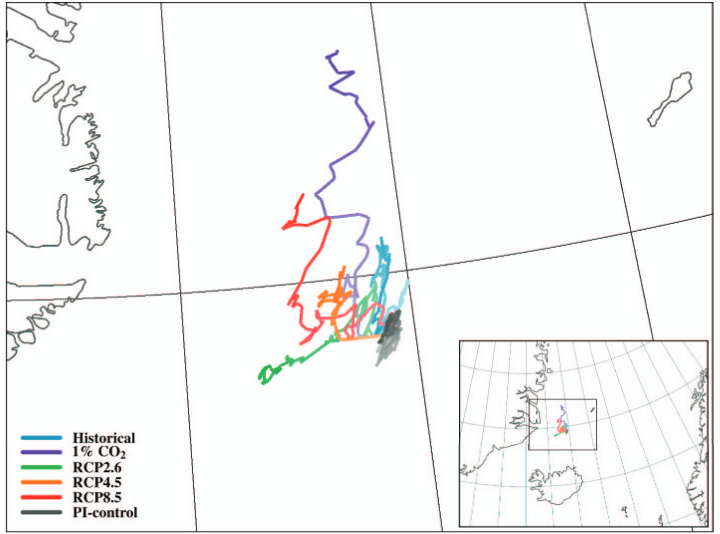
\includegraphics[width=.5 \columnwidth]{imglib/nao_mov_island.png}
      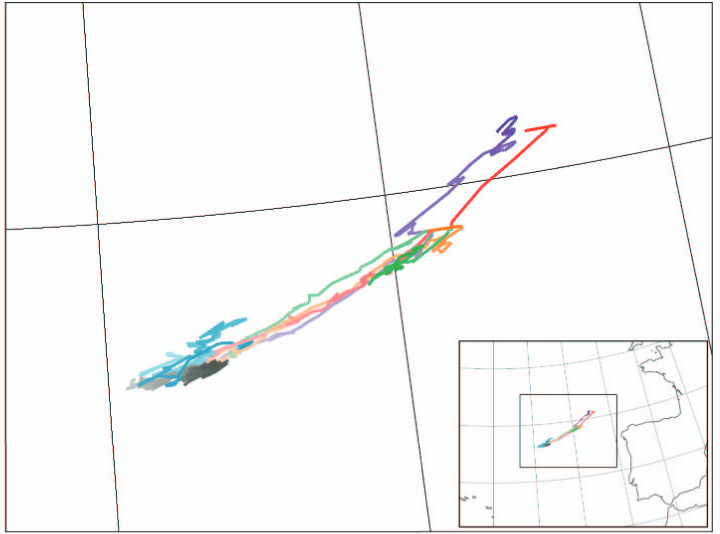
\includegraphics[width=.5 \columnwidth]{imglib/nao_mov_azore.png}
    \end{figure}
      
    \end{column}
    
  \end{columns}
  
\end{frame}


\begin{frame}{Research Questions}
  \begin{center}
    {\huge
      How do the Patterns of Moisture Transport change in the face of various climate scenarios in the North-East Atlantic?
    }
    
  \end{center}  

\end{frame}
